\documentclass[1p]{elsarticle_modified}
%\bibliographystyle{elsarticle-num}

%\usepackage[colorlinks]{hyperref}
%\usepackage{abbrmath_seonhwa} %\Abb, \Ascr, \Acal ,\Abf, \Afrak
\usepackage{amsfonts}
\usepackage{amssymb}
\usepackage{amsmath}
\usepackage{amsthm}
\usepackage{scalefnt}
\usepackage{amsbsy}
\usepackage{kotex}
\usepackage{caption}
\usepackage{subfig}
\usepackage{color}
\usepackage{graphicx}
\usepackage{xcolor} %% white, black, red, green, blue, cyan, magenta, yellow
\usepackage{float}
\usepackage{setspace}
\usepackage{hyperref}

\usepackage{tikz}
\usetikzlibrary{arrows}

\usepackage{multirow}
\usepackage{array} % fixed length table
\usepackage{hhline}

%%%%%%%%%%%%%%%%%%%%%
\makeatletter
\renewcommand*\env@matrix[1][\arraystretch]{%
	\edef\arraystretch{#1}%
	\hskip -\arraycolsep
	\let\@ifnextchar\new@ifnextchar
	\array{*\c@MaxMatrixCols c}}
\makeatother %https://tex.stackexchange.com/questions/14071/how-can-i-increase-the-line-spacing-in-a-matrix
%%%%%%%%%%%%%%%

\usepackage[normalem]{ulem}

\newcommand{\msout}[1]{\ifmmode\text{\sout{\ensuremath{#1}}}\else\sout{#1}\fi}
%SOURCE: \msout is \stkout macro in https://tex.stackexchange.com/questions/20609/strikeout-in-math-mode

\newcommand{\cancel}[1]{
	\ifmmode
	{\color{red}\msout{#1}}
	\else
	{\color{red}\sout{#1}}
	\fi
}

\newcommand{\add}[1]{
	{\color{blue}\uwave{#1}}
}

\newcommand{\replace}[2]{
	\ifmmode
	{\color{red}\msout{#1}}{\color{blue}\uwave{#2}}
	\else
	{\color{red}\sout{#1}}{\color{blue}\uwave{#2}}
	\fi
}

\newcommand{\Sol}{\mathcal{S}} %segment
\newcommand{\D}{D} %diagram
\newcommand{\A}{\mathcal{A}} %arc


%%%%%%%%%%%%%%%%%%%%%%%%%%%%%5 test

\def\sl{\operatorname{\textup{SL}}(2,\Cbb)}
\def\psl{\operatorname{\textup{PSL}}(2,\Cbb)}
\def\quan{\mkern 1mu \triangleright \mkern 1mu}

\theoremstyle{definition}
\newtheorem{thm}{Theorem}[section]
\newtheorem{prop}[thm]{Proposition}
\newtheorem{lem}[thm]{Lemma}
\newtheorem{ques}[thm]{Question}
\newtheorem{cor}[thm]{Corollary}
\newtheorem{defn}[thm]{Definition}
\newtheorem{exam}[thm]{Example}
\newtheorem{rmk}[thm]{Remark}
\newtheorem{alg}[thm]{Algorithm}

\newcommand{\I}{\sqrt{-1}}
\begin{document}

%\begin{frontmatter}
%
%\title{Boundary parabolic representations of knots up to 8 crossings}
%
%%% Group authors per affiliation:
%\author{Yunhi Cho} 
%\address{Department of Mathematics, University of Seoul, Seoul, Korea}
%\ead{yhcho@uos.ac.kr}
%
%
%\author{Seonhwa Kim} %\fnref{s_kim}}
%\address{Center for Geometry and Physics, Institute for Basic Science, Pohang, 37673, Korea}
%\ead{ryeona17@ibs.re.kr}
%
%\author{Hyuk Kim}
%\address{Department of Mathematical Sciences, Seoul National University, Seoul 08826, Korea}
%\ead{hyukkim@snu.ac.kr}
%
%\author{Seokbeom Yoon}
%\address{Department of Mathematical Sciences, Seoul National University, Seoul, 08826,  Korea}
%\ead{sbyoon15@snu.ac.kr}
%
%\begin{abstract}
%We find all boundary parabolic representation of knots up to 8 crossings.
%
%\end{abstract}
%\begin{keyword}
%    \MSC[2010] 57M25 
%\end{keyword}
%
%\end{frontmatter}

%\linenumbers
%\tableofcontents
%
\newcommand\colored[1]{\textcolor{white}{\rule[-0.35ex]{0.8em}{1.4ex}}\kern-0.8em\color{red} #1}%
%\newcommand\colored[1]{\textcolor{white}{ #1}\kern-2.17ex	\textcolor{white}{ #1}\kern-1.81ex	\textcolor{white}{ #1}\kern-2.15ex\color{red}#1	}

{\Large $\underline{12a_{0738}~(K12a_{0738})}$}

\setlength{\tabcolsep}{10pt}
\renewcommand{\arraystretch}{1.6}
\vspace{1cm}\begin{tabular}{m{100pt}>{\centering\arraybackslash}m{274pt}}
\multirow{5}{120pt}{
	\centering
	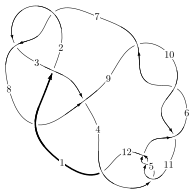
\includegraphics[width=112pt]{../../../GIT/diagram.site/Diagrams/png/1539_12a_0738.png}\\
\ \ \ A knot diagram\footnotemark}&
\allowdisplaybreaks
\textbf{Linearized knot diagam} \\
\cline{2-2}
 &
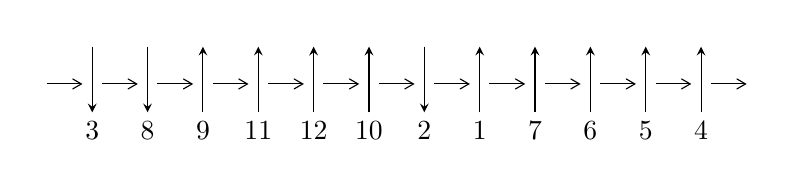
\begin{tikzpicture}[x=20pt, y=17pt]
	% nodes
	\node (C0) at (0, 0) {};
	\node (C1) at (1, 0) {};
	\node (C1U) at (1, +1) {};
	\node (C1D) at (1, -1) {3};

	\node (C2) at (2, 0) {};
	\node (C2U) at (2, +1) {};
	\node (C2D) at (2, -1) {8};

	\node (C3) at (3, 0) {};
	\node (C3U) at (3, +1) {};
	\node (C3D) at (3, -1) {9};

	\node (C4) at (4, 0) {};
	\node (C4U) at (4, +1) {};
	\node (C4D) at (4, -1) {11};

	\node (C5) at (5, 0) {};
	\node (C5U) at (5, +1) {};
	\node (C5D) at (5, -1) {12};

	\node (C6) at (6, 0) {};
	\node (C6U) at (6, +1) {};
	\node (C6D) at (6, -1) {10};

	\node (C7) at (7, 0) {};
	\node (C7U) at (7, +1) {};
	\node (C7D) at (7, -1) {2};

	\node (C8) at (8, 0) {};
	\node (C8U) at (8, +1) {};
	\node (C8D) at (8, -1) {1};

	\node (C9) at (9, 0) {};
	\node (C9U) at (9, +1) {};
	\node (C9D) at (9, -1) {7};

	\node (C10) at (10, 0) {};
	\node (C10U) at (10, +1) {};
	\node (C10D) at (10, -1) {6};

	\node (C11) at (11, 0) {};
	\node (C11U) at (11, +1) {};
	\node (C11D) at (11, -1) {5};

	\node (C12) at (12, 0) {};
	\node (C12U) at (12, +1) {};
	\node (C12D) at (12, -1) {4};
	\node (C13) at (13, 0) {};

	% arrows
	\draw[->,>={angle 60}]
	(C0) edge (C1) (C1) edge (C2) (C2) edge (C3) (C3) edge (C4) (C4) edge (C5) (C5) edge (C6) (C6) edge (C7) (C7) edge (C8) (C8) edge (C9) (C9) edge (C10) (C10) edge (C11) (C11) edge (C12) (C12) edge (C13) ;	\draw[->,>=stealth]
	(C1U) edge (C1D) (C2U) edge (C2D) (C3D) edge (C3U) (C4D) edge (C4U) (C5D) edge (C5U) (C6D) edge (C6U) (C7U) edge (C7D) (C8D) edge (C8U) (C9D) edge (C9U) (C10D) edge (C10U) (C11D) edge (C11U) (C12D) edge (C12U) ;
	\end{tikzpicture} \\
\hhline{~~} \\& 
\textbf{Solving Sequence} \\ \cline{2-2} 
 &
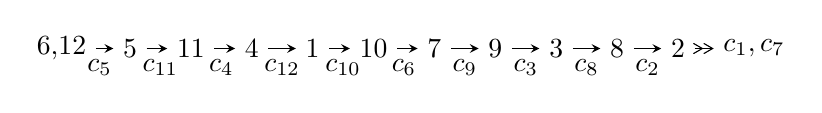
\begin{tikzpicture}[x=22pt, y=7pt]
	% node
	\node (A0) at (-1/8, 0) {6,12};
	\node (A1) at (1, 0) {5};
	\node (A2) at (2, 0) {11};
	\node (A3) at (3, 0) {4};
	\node (A4) at (4, 0) {1};
	\node (A5) at (5, 0) {10};
	\node (A6) at (6, 0) {7};
	\node (A7) at (7, 0) {9};
	\node (A8) at (8, 0) {3};
	\node (A9) at (9, 0) {8};
	\node (A10) at (10, 0) {2};
	\node (C1) at (1/2, -1) {$c_{5}$};
	\node (C2) at (3/2, -1) {$c_{11}$};
	\node (C3) at (5/2, -1) {$c_{4}$};
	\node (C4) at (7/2, -1) {$c_{12}$};
	\node (C5) at (9/2, -1) {$c_{10}$};
	\node (C6) at (11/2, -1) {$c_{6}$};
	\node (C7) at (13/2, -1) {$c_{9}$};
	\node (C8) at (15/2, -1) {$c_{3}$};
	\node (C9) at (17/2, -1) {$c_{8}$};
	\node (C10) at (19/2, -1) {$c_{2}$};
	\node (A11) at (45/4, 0) {$c_{1},c_{7}$};

	% edge
	\draw[->,>=stealth]	
	(A0) edge (A1) (A1) edge (A2) (A2) edge (A3) (A3) edge (A4) (A4) edge (A5) (A5) edge (A6) (A6) edge (A7) (A7) edge (A8) (A8) edge (A9) (A9) edge (A10) ;
	\draw[->>,>={angle 60}]	
	(A10) edge (A11);
\end{tikzpicture} \\ 

\end{tabular} \\

\footnotetext{
The image of knot diagram is generated by the software ``\textbf{Draw programme}" developed by Andrew Bartholomew(\url{http://www.layer8.co.uk/maths/draw/index.htm\#Running-draw}), where we modified some parts for our purpose(\url{https://github.com/CATsTAILs/LinksPainter}).
}\phantom \\ \newline 
\centering \textbf{Ideals for irreducible components\footnotemark of $X_{\text{par}}$} 
 
\begin{align*}
I^u_{1}&=\langle 
u^{59}- u^{58}+\cdots+u^2-1\rangle \\
\\
\end{align*}
\raggedright * 1 irreducible components of $\dim_{\mathbb{C}}=0$, with total 59 representations.\\
\footnotetext{All coefficients of polynomials are rational numbers. But the coefficients are sometimes approximated in decimal forms when there is not enough margin.}
\newpage
\renewcommand{\arraystretch}{1}
\centering \section*{I. $I^u_{1}= \langle u^{59}- u^{58}+\cdots+u^2-1 \rangle$}
\flushleft \textbf{(i) Arc colorings}\\
\begin{tabular}{m{7pt} m{180pt} m{7pt} m{180pt} }
\flushright $a_{6}=$&$\begin{pmatrix}1\\0\end{pmatrix}$ \\
\flushright $a_{12}=$&$\begin{pmatrix}0\\u\end{pmatrix}$ \\
\flushright $a_{5}=$&$\begin{pmatrix}1\\u^2\end{pmatrix}$ \\
\flushright $a_{11}=$&$\begin{pmatrix}- u\\- u^3+u\end{pmatrix}$ \\
\flushright $a_{4}=$&$\begin{pmatrix}- u^2+1\\- u^4+2 u^2\end{pmatrix}$ \\
\flushright $a_{1}=$&$\begin{pmatrix}u^5-2 u^3+u\\u^7-3 u^5+2 u^3+u\end{pmatrix}$ \\
\flushright $a_{10}=$&$\begin{pmatrix}u^3-2 u\\- u^3+u\end{pmatrix}$ \\
\flushright $a_{7}=$&$\begin{pmatrix}u^6-3 u^4+2 u^2+1\\- u^6+2 u^4- u^2\end{pmatrix}$ \\
\flushright $a_{9}=$&$\begin{pmatrix}u^9-4 u^7+5 u^5-3 u\\- u^9+3 u^7-3 u^5+u\end{pmatrix}$ \\
\flushright $a_{3}=$&$\begin{pmatrix}u^{22}-9 u^{20}+\cdots-4 u^2+1\\- u^{22}+8 u^{20}+\cdots+4 u^4+3 u^2\end{pmatrix}$ \\
\flushright $a_{8}=$&$\begin{pmatrix}u^{21}-8 u^{19}+\cdots-4 u^3-3 u\\u^{23}-9 u^{21}+\cdots-4 u^3+u\end{pmatrix}$ \\
\flushright $a_{2}=$&$\begin{pmatrix}- u^{51}+20 u^{49}+\cdots+20 u^5+7 u^3\\u^{51}-19 u^{49}+\cdots- u^3+u\end{pmatrix}$\\&\end{tabular}
\flushleft \textbf{(ii) Obstruction class $= -1$}\\~\\
\flushleft \textbf{(iii) Cusp Shapes $= -4 u^{56}+84 u^{54}+\cdots+8 u+2$}\\~\\
\newpage\renewcommand{\arraystretch}{1}
\flushleft \textbf{(iv) u-Polynomials at the component}\newline \\
\begin{tabular}{m{50pt}|m{274pt}}
Crossings & \hspace{64pt}u-Polynomials at each crossing \\
\hline $$\begin{aligned}c_{1}\end{aligned}$$&$\begin{aligned}
&u^{59}+29 u^{58}+\cdots+2 u+1
\end{aligned}$\\
\hline $$\begin{aligned}c_{2},c_{7}\end{aligned}$$&$\begin{aligned}
&u^{59}+u^{58}+\cdots+u^2-1
\end{aligned}$\\
\hline $$\begin{aligned}c_{3}\end{aligned}$$&$\begin{aligned}
&u^{59}- u^{58}+\cdots-214 u-61
\end{aligned}$\\
\hline $$\begin{aligned}c_{4},c_{5},c_{11}\end{aligned}$$&$\begin{aligned}
&u^{59}- u^{58}+\cdots+u^2-1
\end{aligned}$\\
\hline $$\begin{aligned}c_{6},c_{9},c_{10}\\c_{12}\end{aligned}$$&$\begin{aligned}
&u^{59}+3 u^{58}+\cdots+26 u+5
\end{aligned}$\\
\hline $$\begin{aligned}c_{8}\end{aligned}$$&$\begin{aligned}
&u^{59}+3 u^{58}+\cdots+274 u-187
\end{aligned}$\\
\hline
\end{tabular}\\~\\
\newpage\renewcommand{\arraystretch}{1}
\flushleft \textbf{(v) Riley Polynomials at the component}\newline \\
\begin{tabular}{m{50pt}|m{274pt}}
Crossings & \hspace{64pt}Riley Polynomials at each crossing \\
\hline $$\begin{aligned}c_{1}\end{aligned}$$&$\begin{aligned}
&y^{59}+3 y^{58}+\cdots-18 y-1
\end{aligned}$\\
\hline $$\begin{aligned}c_{2},c_{7}\end{aligned}$$&$\begin{aligned}
&y^{59}-29 y^{58}+\cdots+2 y-1
\end{aligned}$\\
\hline $$\begin{aligned}c_{3}\end{aligned}$$&$\begin{aligned}
&y^{59}+11 y^{58}+\cdots+17370 y-3721
\end{aligned}$\\
\hline $$\begin{aligned}c_{4},c_{5},c_{11}\end{aligned}$$&$\begin{aligned}
&y^{59}-45 y^{58}+\cdots+2 y-1
\end{aligned}$\\
\hline $$\begin{aligned}c_{6},c_{9},c_{10}\\c_{12}\end{aligned}$$&$\begin{aligned}
&y^{59}+71 y^{58}+\cdots-54 y-25
\end{aligned}$\\
\hline $$\begin{aligned}c_{8}\end{aligned}$$&$\begin{aligned}
&y^{59}+23 y^{58}+\cdots-139226 y-34969
\end{aligned}$\\
\hline
\end{tabular}\\~\\
\newpage\flushleft \textbf{(vi) Complex Volumes and Cusp Shapes}
$$\begin{array}{c|c|c}  
\text{Solutions to }I^u_{1}& \I (\text{vol} + \sqrt{-1}CS) & \text{Cusp shape}\\
 \hline 
\begin{aligned}
u &= -1.049650 + 0.244074 I\end{aligned}
 & -1.46822 + 3.88519 I & \phantom{-}2.11458 - 3.15684 I \\ \hline\begin{aligned}
u &= -1.049650 - 0.244074 I\end{aligned}
 & -1.46822 - 3.88519 I & \phantom{-}2.11458 + 3.15684 I \\ \hline\begin{aligned}
u &= -0.015995 + 0.915634 I\end{aligned}
 & -14.7136 - 0.7721 I & -3.56410 - 0.31715 I \\ \hline\begin{aligned}
u &= -0.015995 - 0.915634 I\end{aligned}
 & -14.7136 + 0.7721 I & -3.56410 + 0.31715 I \\ \hline\begin{aligned}
u &= -0.029257 + 0.912896 I\end{aligned}
 & -12.9183 - 9.0890 I & -1.27230 + 5.79658 I \\ \hline\begin{aligned}
u &= -0.029257 - 0.912896 I\end{aligned}
 & -12.9183 + 9.0890 I & -1.27230 - 5.79658 I \\ \hline\begin{aligned}
u &= \phantom{-}0.024127 + 0.908325 I\end{aligned}
 & -10.26760 + 4.09935 I & \phantom{-}1.75919 - 2.25179 I \\ \hline\begin{aligned}
u &= \phantom{-}0.024127 - 0.908325 I\end{aligned}
 & -10.26760 - 4.09935 I & \phantom{-}1.75919 + 2.25179 I \\ \hline\begin{aligned}
u &= \phantom{-}0.008156 + 0.888471 I\end{aligned}
 & -7.74257 + 2.40406 I & \phantom{-}2.67885 - 3.26207 I \\ \hline\begin{aligned}
u &= \phantom{-}0.008156 - 0.888471 I\end{aligned}
 & -7.74257 - 2.40406 I & \phantom{-}2.67885 + 3.26207 I \\ \hline\begin{aligned}
u &= \phantom{-}1.096820 + 0.205121 I\end{aligned}
 & \phantom{-}1.080150 + 0.480738 I & \phantom{-}6.00000 + 0. I\phantom{ +0.000000I} \\ \hline\begin{aligned}
u &= \phantom{-}1.096820 - 0.205121 I\end{aligned}
 & \phantom{-}1.080150 - 0.480738 I & \phantom{-}6.00000 + 0. I\phantom{ +0.000000I} \\ \hline\begin{aligned}
u &= -1.128910 + 0.272160 I\end{aligned}
 & -2.42286 - 3.69043 I & \phantom{-0.000000 } 0 \\ \hline\begin{aligned}
u &= -1.128910 - 0.272160 I\end{aligned}
 & -2.42286 + 3.69043 I & \phantom{-0.000000 } 0 \\ \hline\begin{aligned}
u &= \phantom{-}1.16156\phantom{ +0.000000I}\end{aligned}
 & \phantom{-}2.06866\phantom{ +0.000000I} & \phantom{-}6.00000\phantom{ +0.000000I} \\ \hline\begin{aligned}
u &= \phantom{-}1.269780 + 0.147882 I\end{aligned}
 & \phantom{-}2.98114 - 0.20812 I & \phantom{-0.000000 } 0 \\ \hline\begin{aligned}
u &= \phantom{-}1.269780 - 0.147882 I\end{aligned}
 & \phantom{-}2.98114 + 0.20812 I & \phantom{-0.000000 } 0 \\ \hline\begin{aligned}
u &= \phantom{-}1.256570 + 0.266869 I\end{aligned}
 & -1.39782 + 3.10898 I & \phantom{-0.000000 } 0 \\ \hline\begin{aligned}
u &= \phantom{-}1.256570 - 0.266869 I\end{aligned}
 & -1.39782 - 3.10898 I & \phantom{-0.000000 } 0 \\ \hline\begin{aligned}
u &= -1.272580 + 0.192297 I\end{aligned}
 & \phantom{-}3.97948 - 4.12493 I & \phantom{-0.000000 } 0 \\ \hline\begin{aligned}
u &= -1.272580 - 0.192297 I\end{aligned}
 & \phantom{-}3.97948 + 4.12493 I & \phantom{-0.000000 } 0 \\ \hline\begin{aligned}
u &= -1.292070 + 0.025357 I\end{aligned}
 & \phantom{-}5.86156 - 0.82447 I & \phantom{-0.000000 } 0 \\ \hline\begin{aligned}
u &= -1.292070 - 0.025357 I\end{aligned}
 & \phantom{-}5.86156 + 0.82447 I & \phantom{-0.000000 } 0 \\ \hline\begin{aligned}
u &= \phantom{-}1.303410 + 0.050369 I\end{aligned}
 & \phantom{-}4.08832 + 5.40748 I & \phantom{-0.000000 } 0 \\ \hline\begin{aligned}
u &= \phantom{-}1.303410 - 0.050369 I\end{aligned}
 & \phantom{-}4.08832 - 5.40748 I & \phantom{-0.000000 } 0 \\ \hline\begin{aligned}
u &= -1.284990 + 0.240189 I\end{aligned}
 & \phantom{-}2.75808 - 5.72388 I & \phantom{-0.000000 } 0 \\ \hline\begin{aligned}
u &= -1.284990 - 0.240189 I\end{aligned}
 & \phantom{-}2.75808 + 5.72388 I & \phantom{-0.000000 } 0 \\ \hline\begin{aligned}
u &= \phantom{-}1.296950 + 0.252884 I\end{aligned}
 & \phantom{-}0.47013 + 10.52840 I & \phantom{-0.000000 } 0 \\ \hline\begin{aligned}
u &= \phantom{-}1.296950 - 0.252884 I\end{aligned}
 & \phantom{-}0.47013 - 10.52840 I & \phantom{-0.000000 } 0 \\ \hline\begin{aligned}
u &= -0.154537 + 0.652088 I\end{aligned}
 & -4.02672 - 7.30062 I & -0.57198 + 8.02266 I\\
 \hline 
 \end{array}$$\newpage$$\begin{array}{c|c|c}  
\text{Solutions to }I^u_{1}& \I (\text{vol} + \sqrt{-1}CS) & \text{Cusp shape}\\
 \hline 
\begin{aligned}
u &= -0.154537 - 0.652088 I\end{aligned}
 & -4.02672 + 7.30062 I & -0.57198 - 8.02266 I \\ \hline\begin{aligned}
u &= -0.082927 + 0.664867 I\end{aligned}
 & -5.50022 + 0.23449 I & -3.62552 + 0.57133 I \\ \hline\begin{aligned}
u &= -0.082927 - 0.664867 I\end{aligned}
 & -5.50022 - 0.23449 I & -3.62552 - 0.57133 I \\ \hline\begin{aligned}
u &= -1.261370 + 0.449534 I\end{aligned}
 & -9.10474 + 4.22835 I & \phantom{-0.000000 } 0 \\ \hline\begin{aligned}
u &= -1.261370 - 0.449534 I\end{aligned}
 & -9.10474 - 4.22835 I & \phantom{-0.000000 } 0 \\ \hline\begin{aligned}
u &= \phantom{-}1.264440 + 0.443767 I\end{aligned}
 & -6.42613 + 0.72715 I & \phantom{-0.000000 } 0 \\ \hline\begin{aligned}
u &= \phantom{-}1.264440 - 0.443767 I\end{aligned}
 & -6.42613 - 0.72715 I & \phantom{-0.000000 } 0 \\ \hline\begin{aligned}
u &= \phantom{-}1.273510 + 0.421789 I\end{aligned}
 & -3.81526 + 2.28316 I & \phantom{-0.000000 } 0 \\ \hline\begin{aligned}
u &= \phantom{-}1.273510 - 0.421789 I\end{aligned}
 & -3.81526 - 2.28316 I & \phantom{-0.000000 } 0 \\ \hline\begin{aligned}
u &= -1.273610 + 0.447529 I\end{aligned}
 & -10.81480 - 4.09220 I & \phantom{-0.000000 } 0 \\ \hline\begin{aligned}
u &= -1.273610 - 0.447529 I\end{aligned}
 & -10.81480 + 4.09220 I & \phantom{-0.000000 } 0 \\ \hline\begin{aligned}
u &= -1.286810 + 0.419585 I\end{aligned}
 & -3.71576 - 7.08524 I & \phantom{-0.000000 } 0 \\ \hline\begin{aligned}
u &= -1.286810 - 0.419585 I\end{aligned}
 & -3.71576 + 7.08524 I & \phantom{-0.000000 } 0 \\ \hline\begin{aligned}
u &= \phantom{-}0.135360 + 0.620016 I\end{aligned}
 & -1.62134 + 2.64544 I & \phantom{-}2.55643 - 4.49292 I \\ \hline\begin{aligned}
u &= \phantom{-}0.135360 - 0.620016 I\end{aligned}
 & -1.62134 - 2.64544 I & \phantom{-}2.55643 + 4.49292 I \\ \hline\begin{aligned}
u &= \phantom{-}1.298440 + 0.437752 I\end{aligned}
 & -10.62320 + 5.60619 I & \phantom{-0.000000 } 0 \\ \hline\begin{aligned}
u &= \phantom{-}1.298440 - 0.437752 I\end{aligned}
 & -10.62320 - 5.60619 I & \phantom{-0.000000 } 0 \\ \hline\begin{aligned}
u &= -1.302440 + 0.430305 I\end{aligned}
 & -6.13573 - 8.88432 I & \phantom{-0.000000 } 0 \\ \hline\begin{aligned}
u &= -1.302440 - 0.430305 I\end{aligned}
 & -6.13573 + 8.88432 I & \phantom{-0.000000 } 0 \\ \hline\begin{aligned}
u &= \phantom{-}1.307160 + 0.432172 I\end{aligned}
 & -8.7535 + 13.8960 I & \phantom{-0.000000 } 0 \\ \hline\begin{aligned}
u &= \phantom{-}1.307160 - 0.432172 I\end{aligned}
 & -8.7535 - 13.8960 I & \phantom{-0.000000 } 0 \\ \hline\begin{aligned}
u &= \phantom{-}0.143619 + 0.486456 I\end{aligned}
 & -0.31966 + 1.64759 I & \phantom{-}3.71266 - 6.34085 I \\ \hline\begin{aligned}
u &= \phantom{-}0.143619 - 0.486456 I\end{aligned}
 & -0.31966 - 1.64759 I & \phantom{-}3.71266 + 6.34085 I \\ \hline\begin{aligned}
u &= -0.436286 + 0.252853 I\end{aligned}
 & -1.03116 - 4.55655 I & \phantom{-}4.61891 + 7.76047 I \\ \hline\begin{aligned}
u &= -0.436286 - 0.252853 I\end{aligned}
 & -1.03116 + 4.55655 I & \phantom{-}4.61891 - 7.76047 I \\ \hline\begin{aligned}
u &= -0.280522 + 0.375413 I\end{aligned}
 & -1.54969 + 2.03091 I & \phantom{-}2.13878 + 1.09449 I \\ \hline\begin{aligned}
u &= -0.280522 - 0.375413 I\end{aligned}
 & -1.54969 - 2.03091 I & \phantom{-}2.13878 - 1.09449 I \\ \hline\begin{aligned}
u &= \phantom{-}0.392822 + 0.121836 I\end{aligned}
 & \phantom{-}0.952284 + 0.399884 I & \phantom{-}10.51926 - 2.51736 I \\ \hline\begin{aligned}
u &= \phantom{-}0.392822 - 0.121836 I\end{aligned}
 & \phantom{-}0.952284 - 0.399884 I & \phantom{-}10.51926 + 2.51736 I\\
 \hline 
 \end{array}$$\newpage
\newpage\renewcommand{\arraystretch}{1}
\centering \section*{ II. u-Polynomials}
\begin{tabular}{m{50pt}|m{274pt}}
Crossings & \hspace{64pt}u-Polynomials at each crossing \\
\hline $$\begin{aligned}c_{1}\end{aligned}$$&$\begin{aligned}
&u^{59}+29 u^{58}+\cdots+2 u+1
\end{aligned}$\\
\hline $$\begin{aligned}c_{2},c_{7}\end{aligned}$$&$\begin{aligned}
&u^{59}+u^{58}+\cdots+u^2-1
\end{aligned}$\\
\hline $$\begin{aligned}c_{3}\end{aligned}$$&$\begin{aligned}
&u^{59}- u^{58}+\cdots-214 u-61
\end{aligned}$\\
\hline $$\begin{aligned}c_{4},c_{5},c_{11}\end{aligned}$$&$\begin{aligned}
&u^{59}- u^{58}+\cdots+u^2-1
\end{aligned}$\\
\hline $$\begin{aligned}c_{6},c_{9},c_{10}\\c_{12}\end{aligned}$$&$\begin{aligned}
&u^{59}+3 u^{58}+\cdots+26 u+5
\end{aligned}$\\
\hline $$\begin{aligned}c_{8}\end{aligned}$$&$\begin{aligned}
&u^{59}+3 u^{58}+\cdots+274 u-187
\end{aligned}$\\
\hline
\end{tabular}\newpage\renewcommand{\arraystretch}{1}
\centering \section*{ III. Riley Polynomials}
\begin{tabular}{m{50pt}|m{274pt}}
Crossings & \hspace{64pt}Riley Polynomials at each crossing \\
\hline $$\begin{aligned}c_{1}\end{aligned}$$&$\begin{aligned}
&y^{59}+3 y^{58}+\cdots-18 y-1
\end{aligned}$\\
\hline $$\begin{aligned}c_{2},c_{7}\end{aligned}$$&$\begin{aligned}
&y^{59}-29 y^{58}+\cdots+2 y-1
\end{aligned}$\\
\hline $$\begin{aligned}c_{3}\end{aligned}$$&$\begin{aligned}
&y^{59}+11 y^{58}+\cdots+17370 y-3721
\end{aligned}$\\
\hline $$\begin{aligned}c_{4},c_{5},c_{11}\end{aligned}$$&$\begin{aligned}
&y^{59}-45 y^{58}+\cdots+2 y-1
\end{aligned}$\\
\hline $$\begin{aligned}c_{6},c_{9},c_{10}\\c_{12}\end{aligned}$$&$\begin{aligned}
&y^{59}+71 y^{58}+\cdots-54 y-25
\end{aligned}$\\
\hline $$\begin{aligned}c_{8}\end{aligned}$$&$\begin{aligned}
&y^{59}+23 y^{58}+\cdots-139226 y-34969
\end{aligned}$\\
\hline
\end{tabular}
\vskip 2pc
\end{document}